\documentclass{article}
\usepackage[a4paper, total={6.5in, 10in}]{geometry}
\setlength{\parindent}{0pt}
\usepackage{tcolorbox}
\tcbset{colback=white!94!black, colframe=black!60!white, coltitle = white, boxrule=0.8pt, arc=2mm}
\newtcolorbox{boxs}[2][]{title= #2,#1}
\usepackage{datetime2}
\usepackage[british]{babel}
\usepackage{amsfonts}
\usepackage{amsmath}
\usepackage{pgfplots}
\usepgfplotslibrary{statistics}
\pgfplotsset{compat = 1.18}

\title{\textbf{Statistics HW}}
\author{Robert O'Connell}
\date{\today}
\begin{document}
\maketitle
\vspace{5mm}

\subsection*{Question 1}

\subsubsection*{\((\alpha)\)}
\begin{figure}[h]
\centering
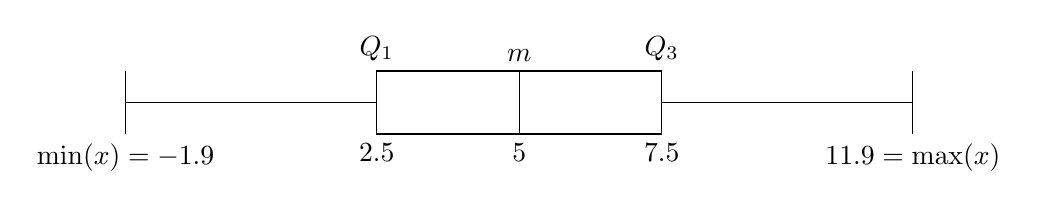
\begin{tikzpicture}
  % Whiskers
  \draw (0,0) -- (3.19,0);
  \draw (6.81,0) -- (10,0);

  % Whisker caps
  \draw (0,-0.4) -- (0,0.4);
  \draw (10,-0.4) -- (10,0.4);

  % Box Q1 to Q3
  \draw (3.19,-0.4) rectangle (6.81,0.4);

  % Median line
  \draw (5.0,-0.4) -- (5.0,0.4);

  % Below labels
  \node[below] at (0,-0.4)    {$\min(x) = -1.9$};
  \node[below] at (3.19,-0.4) {$2.5$};
  \node[below] at (5.0,-0.4)  {$5$};
  \node[below] at (6.81,-0.4) {$7.5$};
  \node[below] at (10,-0.4)   {$11.9 = \max(x)$};

  % Above labels
  \node[above] at (3.19,0.4) {$Q_{1}$};
  \node[above] at (5.0,0.4)  {$m$};
  \node[above] at (6.81,0.4) {$Q_{3}$};
\end{tikzpicture}
\end{figure}

\subsubsection*{\((\beta)\)}
\begin{table}[h]
\centering
\begin{tabular}{|c|c|}
\hline
\textbf{Class} & \textbf{Frequency} \\
\hline
$[-2, 0)$  & 4  \\
$[0, 2)$   & 6  \\
$[2, 4)$   & 8  \\
$[4, 6)$   & 14 \\
$[6, 8)$   & 7  \\
$[8, 10)$  & 8  \\
$[10, 12]$ & 3  \\
\hline
\textbf{Total} & \textbf{50} \\
\hline
\end{tabular}
\end{table}

\begin{figure}[h]
\centering
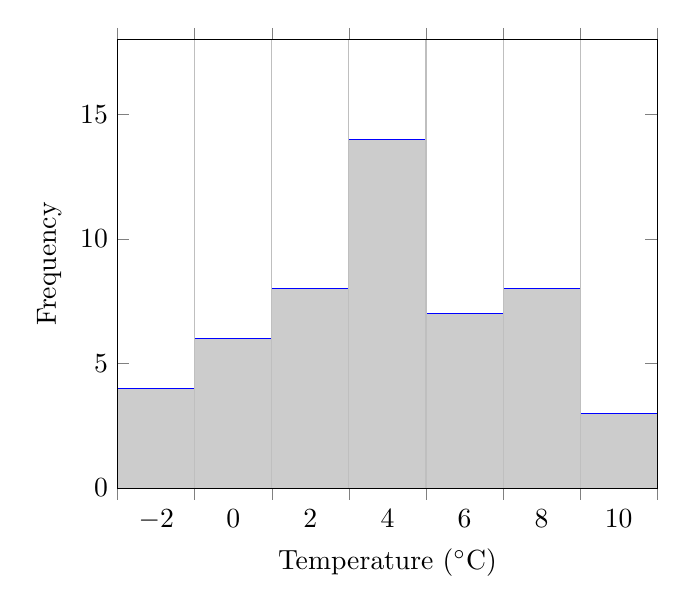
\begin{tikzpicture}
\begin{axis}[
  ymin=0, ymax=18,
  xmin=-2, xmax=12,
  xtick={-2,0,2,4,6,8,10,12},
  xlabel={Temperature ($^\circ$C)},
  ylabel={Frequency},
  bar width=2cm,
  ybar interval,
  area style,
]
\addplot+[fill=gray!40] coordinates {
  (-2, 4)
  (0,  6)
  (2,  8)
  (4,  14)
  (6,  7)
  (8,  8)
  (10, 3)
  (12, 0)
};
\end{axis}
\end{tikzpicture}
\end{figure}

\subsubsection*{\((\gamma)\)}
Mean: \(\frac{1}{50}(-4 + 6 + 24 + 70 + 49 +72 +33) = 5\)

Variance: \(\frac{1}{49}(4(6)^2 + 6(4)^2 + 8(2)^2 + 7(2)^2 + 8(4)^2 + 3(6)^2) = 10.939\)

\subsubsection*{\((\delta)\)}
\begin{itemize}
	\item \(x=0\), which is the fifth datapoint, and is not the average of any two consecutive datapoints,
	thus \(50p = (4,5) \Rightarrow p = (0.08,0.1)\)

	\item \(x = 6\), the only way to get \(6\) is for it be to the average of the 32nd and 33rd datapoint,
	thus \(50p = 32 \Rightarrow p = 0.64\)

	\item \(x=4\), which is the 19th, 20th and 21st datapoint, and is not the average of any two consecutive datapoints other 
	than the fours,
	thus \(50p = [18,21) \Rightarrow p = [0.36, 0.42)\)
\end{itemize}



\subsection*{Question 2}
\subsubsection*{\((\alpha)\)}
Both of these sampling statistics are normally distributed as a result of the
Central Limit Theorem
\[
	S_{100} \approx \mathcal{N}(n \mu , n \sigma ^2) = \mathcal{N}(200 000, 16 000 000)
\]
\[
	\bar{X} \approx \mathcal{N}(\mu, \frac{\sigma^2}{n}) = \mathcal{N}(2 000, 1600)
\]

\subsubsection*{\((\beta)\)}
\begin{itemize}
	\item \(\mathbb{P}(Z < \frac{2049.2 - 2000}{40}) = \mathbb{P}(Z < 1.23) = 0.8907\)
	\item \(\mathbb{P}(Z > \frac{1980-2000}{40}) = 1- \mathbb{P}(Z < - 0.5) = \mathbb{P}(Z < 0.5) = 0.6915\)
\end{itemize}

\subsubsection*{\((\gamma)\)}
\[
	\mathbb{P}(\frac{196000- 200000}{4000} < Z < \frac{208000 - 200000}{4000})
	= \mathbb{P}(-1 < Z < 2 )
\]
\[= \mathbb{P}(Z < 2) -(1 -\mathbb{P}( Z< 1))
	= 0.9772 - ( 1- 0.8413) = 0.8185
\]

\subsubsection*{\((\delta)\)}
\[
	Y_m \approx \mathcal{N}(2000, \frac{16000}{m})
\]

\[
	\mathbb{P}(\bar{Y} > 2030) = 1 - \mathbb{P}(\bar{Y} < 2030)
\]
\[
	\Rightarrow \mathbb{P}(\bar{Y} < 2030) = 0.93319
\]
\[
	\Rightarrow \mathbb{P}\left(Z < \frac{2030- 2000}{\left(\frac{400}{\sqrt{m}}\right)}\right) = 0.93319
\]
\[
	\Rightarrow \frac{30}{\left(\frac{400}{\sqrt{m}}\right)} = 1.5
\]
\[
	\Rightarrow m = 400
\]


\subsection*{Question 3}
\subsubsection*{\((\alpha)\)}
\[
	\bar{x} =  \frac{1}{16} \sum_{i=1}^{16} x_i = 12
\]
\[
	s = \sqrt{\frac{1}{15} \sum_{i=1}^{16} (x_i - \bar{x})^2} = 4
\]

\subsubsection*{\((\beta)\)}
Since we are dealing with a sampling from a normal distrubtion, with both
\(\mu\) and \(\sigma^2\) unknown, the only method at our disposal to
estimate \(\mu\) is the student distrubtion
\[
	(\bar{x} - t_{n-1;\alpha/2}\frac{s}{\sqrt{n}} < \mu < \bar{x} + t_{n-1;\alpha/2}\frac{s}{\sqrt{n}} )
\]
\begin{itemize}
	\item \((12 - 1.753 < \mu < 12 + 1.753) = (10.247 < \mu < 13.753)\)
	\item \((12 - 2.131 < \mu < 12 + 2.131) = (9.869 < \mu < 14.131)\)
\end{itemize}

\subsubsection*{\((\gamma)\)}
\begin{itemize}
	\item \(9\)
	      \begin{itemize}
		      \item Doesn't belong to the \(88\%\)
		      \item Doesn't belong to the \(92\%\)
		      \item Cannot be sure about the \(98\%\)
	      \end{itemize}
	\item \(10\)
	      \begin{itemize}
		      \item Doesn't belong to the \(88\%\)
		      \item Doesn't belong to the \(92\%\)
		      \item Belongs to the \(98\%\)
	      \end{itemize}
	\item \(11\)
	      \begin{itemize}
		      \item Cannot be sure about the \(88\%\)
		      \item Belongs to the \(92\%\)
		      \item Belongs to the \(98\%\)
	      \end{itemize}
\end{itemize}

\subsubsection*{\((\delta)\)}
Now, when the standard deivation is known we can apply the formula
\[
	(\bar{x} - z_{\alpha/2}\frac{\sigma}{\sqrt{n}} < \mu < \bar{x} + z_{\alpha/2}\frac{\sigma}{\sqrt{n}} )
\]
Thus the \(95\%\) confidence interval is
\[
	(12 - 1.96 < \mu < 12 + 1.96) = (10.355 < \mu < 13.645)
\]

The length of a confidence interval is given by
\[
	l = 2z_{\alpha/2}\frac{\sigma}{\sqrt{m}}
\]
Solving for \(m\) for an \(95\%\) confidence interval of at most length \(l_0\), we get
\[
	m \geq \left(\frac{15.68}{l_0}\right)
\]

For \(l_0 = 3\), and \(l_0 = 2\), we get
\[
	m \geq 5.23, \quad m \geq 7.84
\]
Then for \(2\leq l_0 \leq 3\), we have \( 6 \leq m \leq 7\)

\subsection*{Question 4}
\subsubsection*{\((\alpha)\)}
\[
	\hat{p_1} = \frac{3}{5}, \quad \hat{p_2} = \frac{1}{2}
\]

\subsubsection*{\((\beta)\)}
The \(100(1- \alpha)\%\) confidence interval for the percentage \(p\) of a characteristic
is given by
\[
	p \pm z_{\alpha/2}\sqrt{\frac{\hat{p}(1- \hat{p})}{n}}
\]
\begin{itemize}
	\item Then \((0.6 - 1.96\sqrt{\frac{(0.6)(0.4)}{50}} < p_1 < 0.6 + 1.96 \sqrt{\frac{(0.6)(0.4)}{50}})
	      = (0.464 < p_1 < 0.736)\)
	\item Also \((0.5 - 1.645 \sqrt{\frac{0.5^2}{40}} < p_2 < 0.5 + 1.645 \sqrt{\frac{0.5^2}{40}})
	      = (0.370 < p < 0.630)\)
\end{itemize}

\subsubsection*{\((\gamma)\)}
\[
	\hat{p_1} - \hat{p_2} \pm z_{\alpha/2} \sqrt{\frac{\hat{p_1}(1 - \hat{p_1})}{n_1} + \frac{\hat{p_2}(1-\hat{p_2})}{n_2}}
\]

\begin{itemize}
	\item \(\left(0.1 - 2.576\sqrt{\frac{(0.6)(0.4)}{50}+ \frac{0.5^2}{40}} < \hat{p_1} - \hat{p_2} < 0.1 + 2.576\sqrt{\frac{(0.6)(0.4)}{50}+ \frac{0.5^2}{40}}\right)\)
	      \\
	      \(= (-0.171 < \hat{p_1} - \hat{p_2} < 0.371)\)
	      \\

	\item \(\left(-0.1 - 1.96\sqrt{\frac{(0.6)(0.4)}{50}+ \frac{0.5^2}{40}} < \hat{p_2} - \hat{p_1} < -0.1 + 1.96\sqrt{\frac{(0.6)(0.4)}{50}+ \frac{0.5^2}{40}} \right)\)
	      \\
	      \(= ( -0.306 < \hat{p_2} - \hat{p_1} < 0.106)\)
\end{itemize}





\subsubsection*{\((\delta)\)}
We recall the formula for the \(100(1- \alpha)\%\) confidence interval for the
percentage \(p\) of a characteristic
\[
	p \pm z_{\alpha/2}\sqrt{\frac{\hat{p}(1- \hat{p})}{n}}
\]
Then for the characteristic \(q\), we get
\[
	1 - p \pm z_{\alpha/2}\sqrt{\frac{(1-\hat{p})\hat{p}}{n}}
\]

We note that the length of \(C_p\) and \(C_ q\) are the same since
we are adding and subtracting the same term from both of the start points
\(p\) and \(q = 1-p\). These are the same terms since we are dealing with the same dataset and each occurence
of the data is either \(p\) or \(q\)
\\

Moreover, the two confidence intervals are both of equal distance away from
\(p = 0.5\), as a result of the property that \(q = 1-p\)

\subsection*{Question 5}
\subsubsection*{(A)}

\begin{align*}
	g(\theta ; x_1, \dots, x_n) & = f_{X_1}(x_1) f_{X_2}(x_2) \dots f_{X_n}(x_n) \\
	                            & = \theta^n \prod_{i=1}^{n} x_i^{-(1+ \theta)}
\end{align*}

To maximise the likelihood, it suffices to do it for the log of the function
\begin{align*}
	h(\theta) & = \ln(g(\theta; X_1 \dots X_n))                  \\
	          & = n\ln\theta - (1+\theta) \sum_{i=1}^{n} \ln X_i
\end{align*}
\[
	h'(\theta) = \frac{n}{\theta} - \sum_{i=1}^{n} \ln X_i
\]

When \(h'(\hat{\theta}) = 0\), we have
\[
	\frac{n}{\hat{\theta}} = \sum_{i=1}^{n} \ln X_i
\]
\[
	\Rightarrow \hat{\theta} = \frac{n}{\sum_{i=1}^{n} Y_i}
\]

To check whether this is a maximum or not we look at the second derivative of \(h(\theta)\)
\[
	h''(\theta) = -\frac{n}{\theta^2}
\]
\[
	h''(\hat{\theta}) = -\frac{n}{\hat{\theta^2}}
\]
Since \(n > 0\) and \(\hat{\theta}^2 > 0\), we have that this is indeed a maximum and thus
\[
	\text{MLE}(\theta) = \hat{\theta} = \frac{n}{\sum_{i=1}^{n} Y_i} = \frac{1}{\bar{Y}}
\]

\subsubsection*{(B)}
\begin{itemize}
	\item \[
		      \bar{x} = \frac{x_1 + \dots + x_n}{n}, \quad \bar{y} = \frac{y_1 + \dots + y_m}{m}
	      \]
	      Let \(z = \{x_1, \dots, x_n, y_1, \dots y_m\}\)
	      \begin{align*}
		      \bar{z} & = \frac{x_1 + \dots + x_n + y_1 + \dots + y_m}{n+m} \\
		              & = \frac{n\bar{x} + m\bar{y}}{n+m}
	      \end{align*}
	\\

	\item \[
		  	s_x^2  =\frac{1}{n-1} \sum_{i=1}^{n} (x_i - \bar{x})^2, \quad s_y^2 = \frac{1}{m-1} \sum_{i=1}^{m} (y_i - \bar{y})^2
		\]
	Then 
	\begin{align*}
	s^2 &= \frac{1}{n+m-1} \sum_{i=1}^{n+m} (z_i - \bar{z})^2 \\
	&= \frac{1}{n+m-1} ( \sum_{i=1}^{n} (x_i - \bar{z})^2 + \sum_{i=1}^{m}(y_i - \bar{z})^2) \\
	&= \frac{1}{n+m-1} ( \sum_{i=1}^{n} (x_i - \bar{x} + \bar{x} -\bar{z})^2 + \sum_{i=1}^{m}(y_i - \bar{y} + \bar{y} - \bar{z})^2) \\
	&= \frac{1}{n+m-1} ( \sum_{i=1}^{n} (x_i - \bar{x})^2 + 2(\bar{x}- \bar{z})\sum_{i=1}^{n}(x_i - \bar{x}) + n(\bar{x}- \bar{z})^2 + \sum_{i=1}^{m}(y_i - \bar{y})^2 2(\bar{y}- \bar{z})\sum_{i=1}^{n}(y_i - \bar{y}) + m(\bar{y}- \bar{z})^2) \\
	&(\sum_{i=1}^{n} (x_i - \bar{x}) = 0) \ \text{Similarly for y}\\
	&= \frac{1}{n+m-1} ((n-1)s_x^2 + (m-1)s_y^2 + n(\bar{x} - \bar{z})^2 + m(\bar{y} - \bar{z})^2) \\
	&= \frac{1}{n+m-1} ((n-1)s_x^2 + (m-1)s_y^2 + \frac{nm}{n+m}(\bar{x} - \bar{y})^2)
	\end{align*}

\end{itemize}
\subsubsection*{(C)}
\[
f(t) = \sum_{i=1}^{n} |x_i - t|, \quad t \in \mathbb{R}
\]

With \(k\) being the index where the \(x_i\)'s become greater than \(t\), 
we can rewrite this as 
\[
f(t) = \sum_{i=1}^{k} (t - x_i) + \sum_{i= k+1}^{n} (x_i - t)
\]

Then
\[
f'(t) = k - (n-k) = 2k - n
\]

Now let \(m = \frac{n+1}{2}\). Since \(n\) is odd, \(x_m\) is the median of the dataset.

If \(t < x_m\), then \(k < m\), so
\[
f'(t) = 2k - n < 0
\]
and hence \(f(t)\) is decreasing.

If \(t > x_m\), then \(k \ge m\), so
\[
f'(t) = 2k - n > 0
\]
and hence \(f(t)\) is increasing.

Therefore \(f(t)\) decreases for \(t < x_m\) and increases for \(t > x_m\), so the minimum occurs at
\[
t^* = x_m = x_{\frac{n+1}{2}}.
\]

Thus the value of \(t\) that minimizes \(f(t)\) is the median of the observations.



\subsubsection*{(D)}
\begin{itemize}
	\item Let \( z= \{1,2, \dots, n\}\)

	      Then \( \bar{z} = \frac{1 + 2 + \dots + n}{n} = \frac{n+1}{2}\)

	      We also know that the variance is given by \(\frac{1}{n-1}(\sum i^2) - n(\bar{x})^2\)

	      Thus \( s^2=
\frac{1}{n-1}
\left(
\frac{n(n+1)(2n+1)}{6}
-
n\left(\frac{n+1}{2}\right)^2
\right)
=
\frac{n(n+1)}{12}
\)
	
	\item Then from the Exercise 1.3 we have the sample mean of the new set being added by the constant alpha
	\(\frac{n+1 + 2\alpha}{2}\) and the	sample variance being the same \(\frac{n(n+1)}{12}\)
\end{itemize}

\end{document}
